\chapter{User Manual}

\section{Introduction}

\section{Installation}

\subsection{Prerequisite Installation}
\label{Prerequisite_Installation}

%include as many subsubsections as necessary for each piece of required software
\subsubsection{Installing Python}
\begin{enumerate}
	\item go to https://www.python.org
	\item click the downloads button
	\item click python 3.4.3
\begin{figure}[H]
	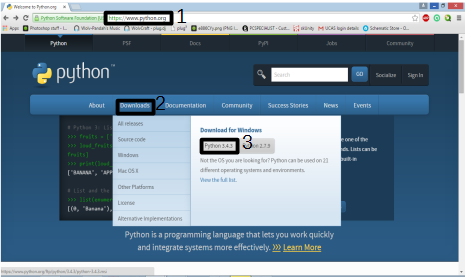
\includegraphics{./manual/images/python-installation-instructions-1.png}
	\caption{How to install python steps 1, 2 and 3}
\end{figure}

	\item navigate to the location the installer was saved to and open it
	
\begin{figure}[H]
	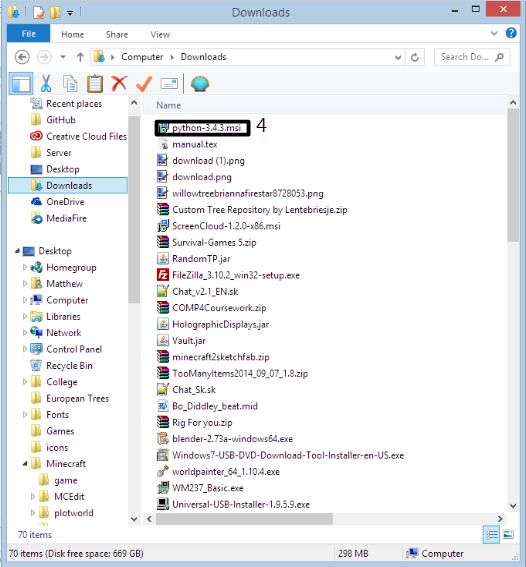
\includegraphics{./manual/images/python-installation-instructions-2.png}
	\caption{How to install python step 4}
\end {figure}

\begin{figure}[H]
	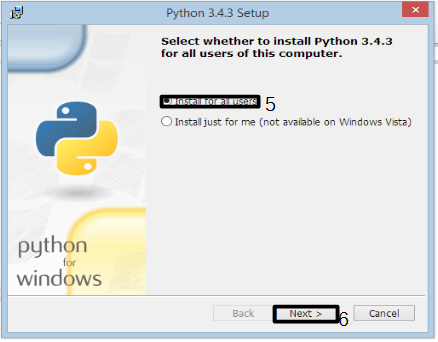
\includegraphics{./manual/images/python-installation-instructions-3.png}
	\caption{How to install python steps 5 and 6}
\end{figure}

\begin{figure}[H]
	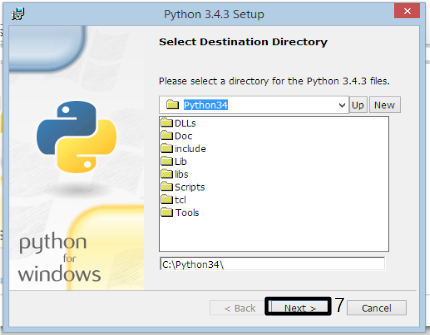
\includegraphics{./manual/images/python-installation-instructions-4.png}
	\caption{How to install python step 7}
\end{figure}

\begin{figure}[H]
	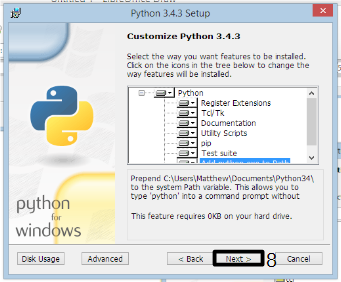
\includegraphics{./manual/images/python-installation-instructions-5.png}
	\caption{How to install python step 8}
\end{figure}

\begin{figure}[H]
	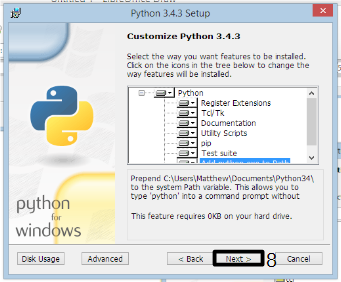
\includegraphics{./manual/images/python-installation-instructions-5.png}
	\caption{How to install python step 9}
\end{figure}
\end{enumerate}

\subsubsection{Installing PyQt}
\begin{enumerate}
	\item go to http://www.riverbankcomputing.co.uk/software/pyqt/download
	\item download the right PyQt .exe file for your system

\begin{figure}[H]
	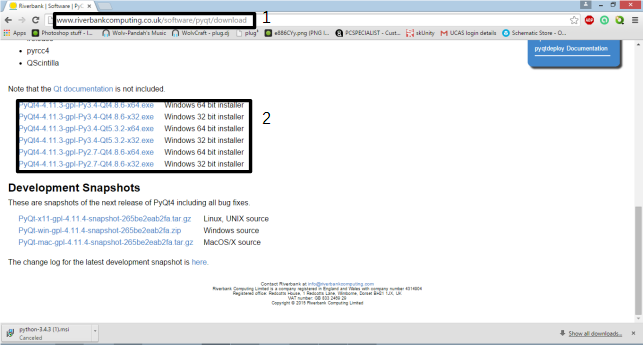
\includegraphics{./manual/images/pyqt-installation-instructions-1.png}
	\caption{How to install python steps 1 and 2}
\end{figure}

	\item navigate to the location of the downloaded .exe file
	
\begin{figure}[H]
	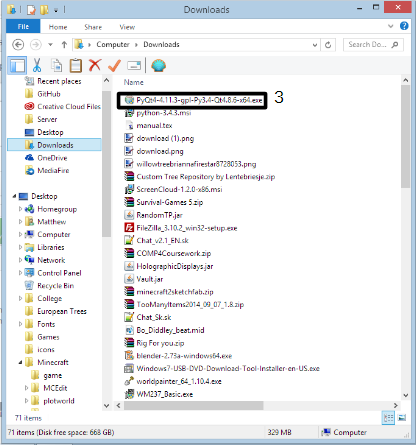
\includegraphics{./manual/images/pyqt-installation-instructions-2.png}
	\caption{How to install python step 3}
\end{figure}

\begin{figure}[H]
	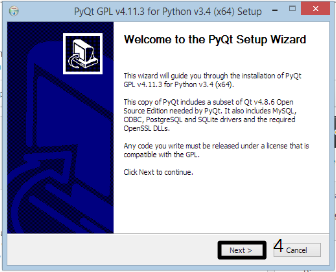
\includegraphics{./manual/images/pyqt-installation-instructions-3.png}
	\caption{How to install python step 4}
\end{figure}

\begin{figure}[H]
	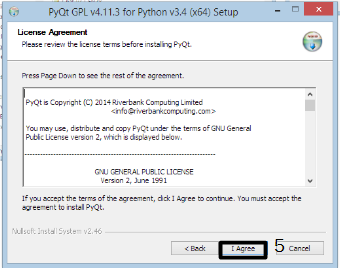
\includegraphics{./manual/images/pyqt-installation-instructions-4.png}
	\caption{How to install python step 5}
\end{figure}

\begin{figure}[H]
	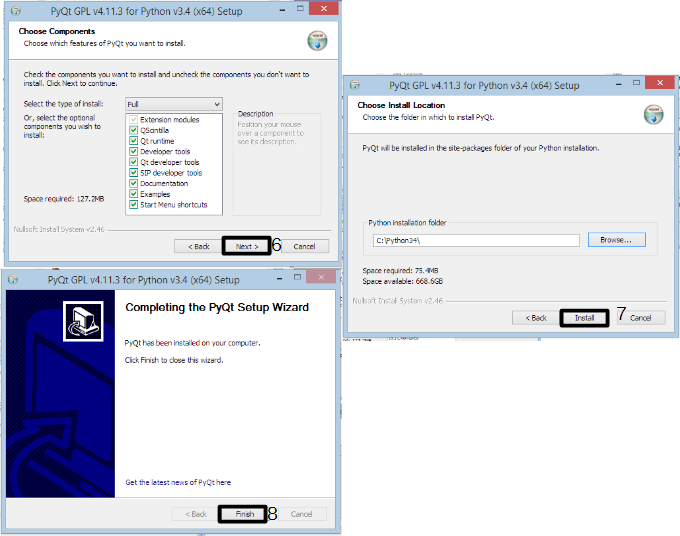
\includegraphics{./manual/images/pyqt-installation-instructions-5.png}
	\caption{How to install python steps 6,7 and 8}
\end{figure}
\end{enumerate}

\subsubsection{Etc.}

\subsection{System Installation}
\label{System_Installation}
\begin{enumerate}
	\item go to https://github.com/MattAnderson16/COMP4Coursework
	\item click the 'Download ZIP' button
	\item navigate to where the downloaded file is saved
	\item open 'COMP4Coursework-master.zip'
	\item open the 'COMP4Coursework-master' folder 
	\item select the 'Implementation' folder
	\item click the 'extract' button
	\item select where you want the folder to be extracted to
	\item click 'OK'
\end{enumerate}

\subsection{Running the System}
\label{Running_the_System}
\begin{enumerate}
	\item navigate to where the system is saved.
	\item open 'new\_main\_window.py'
\end{enumerate}

\section{Tutorial}

\subsection{Introduction}

\subsection{Assumptions}
This tutorial assumes that you already have Python, PyQt4, MatPlotLib and the main system installed (See the prerequisite installation on page \pageref{Prerequisite_Installation} and the system installation on page \pageref{System_Installation} for instructions on how to install these) and that you can open the system (See Running the System on page \pageref{Running_the_System} for instructions on how to open the system.

\subsection{Tutorial Questions}

\subsubsection{How do I add a user?}
To add a user, first click the 'profile' option on the main menu and then click the 'new profile' option. From there, type the first name, last name and password of the user you're adding into the text boxes and click the 'confirm' button.
\begin{figure}[H]
	\includegraphics{./manual/images/system-tutorial-1.png}
	\caption{How to add a user}
\end{figure}

\subsubsection{How do I edit a user?}
To edit a user, first click the 'profile' option on the main menu and then click the 'edit profile' option. From there, select the user you want to edit and type the new first name, new last name and new password into the text boxes and click the 'confirm' button
\begin{figure}[H]
	\includegraphics{./manual/images/system-tutorial-3.png}
	\caption{How to edit a user}
\end{figure}

\subsubsection{How do I remove a user?}
To remove a user, first click the 'profile' option on the main menu and then click the 'remove profile' option. From there, select the user you want to remove and click the 'confirm' button.
\begin{figure}[H]
	\includegraphics{./manual/images/system-tutorial-2.png}
	\caption{How to remove a user}
\end{figure}

\subsubsection{How do I add a reading?}
\begin{figure}[H]
	\includegraphics{./manual/images/system-tutorial-4.png}
	\caption{How to add a reading}
\end{figure}

\subsubsection{How do I edit a reading?}
\begin{figure}[H]
	\includegraphics{./manual/images/system-tutorial-5.png}
	\caption{How to edit a reading}
\end{figure}

\subsubsection{How do I remove a reading?}
\begin{figure}[H]
	\includegraphics{./manual/images/system-tutorial-6.png}
	\caption{How to remove a reading}
\end{figure}

\subsubsection{How do I add a cost?}

\subsubsection{How do I edit a cost?}

\subsubsection{How do I remove a cost?}

\subsubsection{How do I add a type?}

\subsubsection{How do I edit a type?}

\subsubsection{How do I remove a type?}

\subsubsection{How do I refresh a table or graph after data has been added?}
Refreshing a table or graph is as easy as clicking the 'refresh' button above the table.

\subsubsection{How do I view a bar chart?}

\subsubsection{How do I view a pie chart?}

\subsubsection{How do I view different data on the table?}

\subsection{Saving}
The system saves data added to the database automatically once the 'confirm' button is pressed after adding, editing or removing data

\subsection{Limitations}

\section{Error Recovery}

%include as many subsections as necessary for each error
\subsection{Error 1}

\subsection{Error 2}

\section{System Recovery}

\subsection{Backing-up Data}

\subsection{Restoring Data}
